%% ShadowLedger — CIIS 2026 full paper (ACM ICPS / TAPS), target 10--14 pp.
%% Double-blind: `anonymous,review` hides authors + adds review line numbers.
%% Camera-ready: remove `anonymous,review`, fill author block, real CCS + rights.
%%
%% STRUCTURE: each section lives in secciones/NN-name.tex (edit those, not this file).
%% BUILD: pdflatex -> bibtex -> pdflatex x2  (references.bib must be copied to the
%% output dir when using -output-directory; see compile-all.ps1).
\documentclass[sigconf,anonymous,review]{acmart}

\acmConference[CIIS 2026]{IX International Congress on Systems Engineering}{2026}{Lima, Peru}
\settopmatter{printacmref=false}
\renewcommand\footnotetextcopyrightpermission[1]{}
\pagestyle{plain}

%% Figures, plots, pseudocode, listings.
\usepackage{tikz}
\usetikzlibrary{arrows.meta,positioning,fit,backgrounds,calc}
\usepackage{pgfplots}
\pgfplotsset{compat=1.17}
\usepackage[ruled,vlined]{algorithm2e}
\usepackage{listings}
\lstset{basicstyle=\ttfamily\scriptsize,columns=fullflexible,keepspaces=true,
  frame=single,breaklines=true,aboveskip=4pt,belowskip=2pt}

\begin{document}

\title{ShadowLedger: A Storage-Scarce Blockchain with Erasure-Coded Fragmented History and Storage-Weighted Leader Election}

\author{Anonymous Author(s)}
\affiliation{\institution{Submission to CIIS 2026}\country{}}

\begin{abstract}
Full nodes in conventional blockchains must store the \emph{entire} chain history, an
unbounded, monotonically growing cost paid by every node, which centralizes validation
around storage-rich operators and wastes resources through total replication. Proof-of-Work
(PoW) chains compound this with energy spent purely to order blocks. We present
\textbf{ShadowLedger}, a permissionless blockchain in which \emph{storage}, not
computation, is the scarce, security-relevant resource. Every block body is encoded with
Reed--Solomon into $K{+}M$ shards and distributed by rendezvous (highest-random-weight)
hashing, so that \emph{no node stores the full history}: any $K$-of-$(K{+}M)$ shards
reconstruct a block while fewer than $K$ reveal nothing. The right to produce blocks comes
not from hashing but from a Proof-of-Storage discipline over an on-chain, bonded validator
registry, gated against Sybil attacks by a one-shot registration PoW and protected by
equivocation slashing. Leader election is \emph{weighted by proven storage}: validators submit
on-chain storage-proof records for protocol-assigned shards, and a validator's block-production
odds scale with its accepted proofs, decaying to a base weight if it stops proving. We are explicit
about what remains: \emph{bond} slashing for missed proofs (the prototype penalizes by weight
decay, not bond burn) and storage-weighted \emph{fork choice} (branch weight is still chain length)
are documented gaps, not hidden ones. A heaviest-chain fork-choice and reorganization engine (state rewind
plus replay) with depth-based finality provides convergence and hard irreversibility, and a
PoW faucet anchored to committed block data lets capital-less newcomers join. We give the
design, an analytical model showing per-node history storage scales as $O(1/n)$ in the
number of nodes $n$, and measurements from a running Go prototype deployed on a public cloud
node: at $n{=}128$ each node stores $\approx 28\times$ less than a full replica; Reed--Solomon
coding sustains $0.3$--$1.4$\,GB/s with a fixed $1.5\times$ overhead; seven forged-block
attack variants are rejected; two partitioned validators reconverge; and a zero-balance
wallet earns its first coins on the live network. We articulate the central
\emph{state-versus-history} separation that reconciles ``no node stores everything'' with
stateless validation, present a threat model, and state the open problems
(storage-weighted fork choice, succinct state commitments, external audit) candidly.
\end{abstract}

\begin{CCSXML}
<ccs2012>
<concept><concept_id>10002978.10003022</concept_id><concept_desc>Security and privacy~Distributed systems security</concept_desc><concept_significance>500</concept_significance></concept>
<concept><concept_id>10003752.10003809.10010172</concept_id><concept_desc>Theory of computation~Distributed algorithms</concept_desc><concept_significance>300</concept_significance></concept>
<concept><concept_id>10002951.10003227</concept_id><concept_desc>Information systems~Data management systems</concept_desc><concept_significance>300</concept_significance></concept>
</ccs2012>
\end{CCSXML}
\ccsdesc[500]{Security and privacy~Distributed systems security}
\ccsdesc[300]{Theory of computation~Distributed algorithms}
\ccsdesc[300]{Information systems~Data management systems}

\keywords{blockchain, erasure coding, Reed--Solomon, rendezvous hashing, proof-of-storage,
data availability, consensus, finality, smart contracts}

\maketitle

\section{Introduction}
A defining and growing cost of operating a full node in Bitcoin~\cite{nakamoto2008bitcoin} or
Ethereum is storing the complete transaction history. This cost is \emph{unbounded}, it
only ever increases, and it is paid by \emph{every} full node, because the classical
security model replicates the whole chain everywhere. The practical consequence is
centralization: as history accumulates, fewer participants can afford to validate
independently, and the network drifts toward a small set of storage-rich operators. Energy
is the second well-known cost: PoW chains expend electricity solely to decide who appends the
next block, work that is intrinsically discarded.

The magnitude is not hypothetical. Production chains accumulate history into the hundreds of
gigabytes and beyond, and the requirement that every validating node retain all of it is widely
recognized as a scalability and decentralization bottleneck, motivating an entire line of
coded-storage work~\cite{yang2024scaling,perard2018erasure}. Yet most such work treats coding as
an optimization bolted onto an unchanged consensus. We instead ask what a chain looks like when
fragmentation is the \emph{default} and when block-production rights are derived from the very act
of storing fragments.

We take the position that the scarce, security-relevant resource of a blockchain should be
\emph{storage of the network's own data}, not wasted hashing, and that \emph{no single node
should need the entire history} to participate. \textbf{ShadowLedger} is our realization of
this position. Its thesis has two parts. First, block \emph{history} is erasure-coded and
scattered across the network so each node retains only a fraction, yet any sufficiently large
set of nodes can reconstruct any block on demand. Second, the right to produce blocks is
earned by \emph{proving storage} of assigned fragments over a bonded validator set, rather
than by burning energy; the only PoW present is a one-shot Sybil gate and a small onboarding
faucet, never the block-ordering mechanism.

Realizing this is not free of tension. If history is not stored whole, validators must still
be able to recover it, or a malicious producer could withhold data; this is the
\emph{data-availability} problem~\cite{albassam2021fraud,yu2020coded}. If block production is
permissionless, the system must resist Sybil flooding and equivocation. And if storage
replaces hashing, the protocol must measure and reward it without a centralized auditor. We
address each of these and report what a working implementation achieves and what it does not.

\paragraph{Contributions.}
\begin{enumerate}
  \item An architecture that fragments \emph{history} (block bodies) with Reed--Solomon coding
  and rendezvous placement while keeping \emph{state} (balances, nonces, contract storage)
  materialized locally, the \emph{state-versus-history} separation that reconciles ``no node
  stores everything'' with fast stateless validation (\S\ref{sec:history}).
  \item A Proof-of-Storage consensus with a bonded on-chain validator registry, a one-shot
  registration PoW as a Sybil gate, HRW leader election with a round-based liveness fallback,
  equivocation slashing, a heaviest-chain reorg engine, and depth-based finality
  (\S\ref{sec:consensus}, \S\ref{sec:fork}). Leader election is weighted by
  on-chain proven storage (validators submit storage-proof records that drive election odds); what
  remains specified-not-built is \emph{bond} slashing for missed proofs (the prototype uses weight
  decay) and storage-weighted \emph{fork choice} (\S\ref{sec:audit}, \S\ref{sec:disc}).
  \item A capital-free onboarding mechanism (a PoW faucet) and a deterministic contract VM with
  a Solidity-like language, both anchored to committed block data and thus verifiable without
  holding the fragmented body (\S\ref{sec:econ}, \S\ref{sec:vm}).
  \item An analytical storage model ($O(1/n)$ per-node history) and an empirical evaluation of a
  live Go prototype, with an explicit threat model and an honest account of open problems
  (\S\ref{sec:threat}--\S\ref{sec:disc}).
\end{enumerate}

The paper is organized as follows. \S\ref{sec:bg} and \S\ref{sec:related} review the primitives
(erasure coding, rendezvous hashing, data availability, storage-based consensus) and position
ShadowLedger against prior coded blockchains, sharding, and proof-of-storage systems.
\S\ref{sec:overview} states the design goals and gives the node architecture. \S\ref{sec:history}
develops the erasure-coded history and its storage model; \S\ref{sec:consensus}--\ref{sec:fork}
the Proof-of-Storage consensus, storage auditing, fork choice, and finality; \S\ref{sec:econ} the
economics and capital-free onboarding; and \S\ref{sec:vm} the contract VM. \S\ref{sec:threat}
presents the threat model, \S\ref{sec:impl} the implementation, and \S\ref{sec:eval} the
evaluation. \S\ref{sec:disc}--\ref{sec:rationale} discuss limitations, applicability, and design
rationale before \S\ref{sec:concl} concludes.

\section{Background}
\label{sec:bg}
\textbf{Reed--Solomon erasure codes.} A Reed--Solomon (RS) code~\cite{reed1960polynomial}
encodes $K$ data symbols into $K{+}M$ symbols such that the original is recoverable from
\emph{any} $K$ of them; it tolerates up to $M$ erasures. Compared with $r$-fold replication
(which costs $r\times$ storage to survive $r{-}1$ losses), an $(K,M)$ RS code survives $M$
losses at only $(K{+}M)/K$ overhead. Crucially, RS is all-or-nothing below the threshold:
fewer than $K$ symbols determine the message no better than zero symbols do, which doubles as
a confidentiality property for partial holders.

\emph{Worked example.} Take $K{=}4,M{=}2$, so $T{=}6$ shards tolerate $M{=}2$ erasures at
$T/K=1.5\times$ overhead. A $1$\,MiB body splits into four $256$\,KiB data shards plus two
$256$\,KiB parity shards; any four of the six rebuild the megabyte. Triple replication would
instead store $3$\,MiB to survive two losses, twice the cost for the same fault tolerance.
This $1.5\times$-versus-$3\times$ gap, generalized over a growing node set, is the lever
ShadowLedger pulls (\S\ref{sec:storagemodel}).

\textbf{Rendezvous (HRW) hashing.} Given a key and a set of nodes, highest-random-weight
hashing~\cite{thaler1998rendezvous} ranks nodes by $h(\text{key},\text{node})$ and assigns the
key to the top-ranked node(s). Unlike ring-based consistent hashing~\cite{karger1997consistent},
each key's ranking is independent, so adding or removing a node reshuffles only the keys that
node would win or lose, ideal for shard placement under churn. Formally, for a key $\kappa$, node
set $V$, and replication $r$, the holders are the top-$r$ nodes by weight,
\[
\textsc{Holders}(\kappa,V,r) \;=\; \operatorname*{top\text{-}}r_{v\in V}\; H(\kappa \,\|\, v),
\]
and a single highest-weight node is the special case $r{=}1$ used for leader election with
$\kappa=(\textit{prevHash},h,t)$. Adding a node $v'$ changes the holder set of $\kappa$ only if
$H(\kappa\|v')$ ranks within the top $r$, so the expected fraction of keys reassigned on a single
join is $r/|V|$, which is the minimal disruption a placement scheme can achieve. We use HRW for
both shard placement and leader election, keeping one source of deterministic, agreement-free
randomness.

\textbf{Data availability.} When blocks are erasure-coded and dispersed, light or partial
nodes need assurance the data \emph{exists} and can be reconstructed. Fraud and
data-availability proofs~\cite{albassam2021fraud}, coded Merkle trees~\cite{yu2020coded}, and
the formal theory of data-availability sampling~\cite{hallandersen2025foundations,hallandersen2024frida}
show that with $2$D/coded commitments a verifier can probabilistically check availability by
sampling a few shards: if a fraction of the coded data is missing, an erasure-coded block cannot
be reconstructed, and that missing fraction is exactly what random sampling is overwhelmingly
likely to hit, so a withholding producer is caught with few queries. These results target
light clients that never store blocks. ShadowLedger's setting is different, its participants
\emph{do} store shards, so it uses a simpler operational notion suited to a fragment-holding
network (\S\ref{sec:history}): a block is canonical only if the network can reconstruct it to its
signed commitment, and a node that needs a body gathers $K$ shards and verifies the hash. Layering
succinct DA sampling on top, to protect non-storing light clients, is compatible and left as
future work.

\textbf{Storage-based consensus.} Replacing PoW's wasted work with a useful resource is a
recurring goal. Proofs of space~\cite{dziembowski2015proofs} and
space-time~\cite{moran2019simple} prove dedicated disk; SpaceMint~\cite{park2018spacemint} and
Chia~\cite{cohen2019chia} build currencies on them. Proofs of
retrievability~\cite{juels2007pors}, proof-of-replication~\cite{fisch2018scaling},
decentralized storage networks such as Storj~\cite{wilkinson2016storj}, and
Permacoin~\cite{miller2014permacoin} bind rewards to stored data. The energy contrast is the
motivation: PoW chains spend electricity per block forever, whereas storing data is a one-time
cost amortized over the data's lifetime, so a storage-based right to produce blocks converts an
ongoing burn into a useful, reusable asset. ShadowLedger's Proof-of-Storage is closest to Permacoin
in spirit but applies to the chain's \emph{own} erasure-coded history rather than an external
archive, so the resource being proved is the very data the network must keep anyway.

\section{Related Work}
\label{sec:related}
\textbf{Coded and low-storage blockchains.} Several systems erasure-code blocks to shrink
per-node storage: low-storage nodes that keep RS fragments~\cite{perard2018erasure}, secure
fountain (LT-code) architectures~\cite{kadhe2019sef}, entropy-based
downsampling~\cite{huang2022downsampling}, and failure-pattern-aware
codes~\cite{mitra2019patterned}; a recent survey maps the field~\cite{yang2024scaling}. These
works typically retain a conventional consensus and treat coding as a storage optimization
layered on top. ShadowLedger instead makes fragmentation the \emph{default} for all history
\emph{and} couples shard placement to the consensus membership set, so storage and
block-production rights are one mechanism rather than two. The closest points of comparison
differ in emphasis: erasure-coded low-storage nodes~\cite{perard2018erasure} keep RS fragments
but rely on a fixed set of full nodes to bootstrap from, and the secure-fountain
architecture~\cite{kadhe2019sef} analyzes precisely the storage-versus-bootstrap-bandwidth
tradeoff we revisit empirically in \S\ref{sec:eval}; coded Merkle trees~\cite{yu2020coded} and
downsampling~\cite{huang2022downsampling} optimize availability proofs and per-node footprint
respectively. None of these ties the act of \emph{storing a shard} to the right to \emph{produce
a block}, which is ShadowLedger's organizing idea.

\textbf{Data-availability designs.} LazyLedger/Celestia~\cite{albassam2019lazyledger} reduces
block validity to data availability; coded Merkle trees~\cite{yu2020coded} and DA
sampling~\cite{hallandersen2025foundations,hallandersen2024frida} give succinct availability
guarantees. ShadowLedger shares the availability-first philosophy but targets a
fragment-storing full-node network rather than a light-client sampling regime; succinct DA
proofs are complementary future work (\S\ref{sec:disc}).

\textbf{Sharding.} Elastico~\cite{luu2016elastico}, OmniLedger~\cite{kokoriskogias2018omniledger},
RapidChain~\cite{zamani2018rapidchain}, and Monoxide~\cite{wang2019monoxide} scale throughput by
partitioning \emph{transactions/state} across committees. ShadowLedger instead partitions
\emph{storage of history} while keeping a single global state and a single ordering, so it does
not inherit cross-shard atomicity costs; the lineage's use of one-shot PoW for committee
randomness directly informs our registration gate.

\textbf{Storage markets versus storage ledgers.} Filecoin~\cite{fisch2018scaling} and
Storj~\cite{wilkinson2016storj} are decentralized storage \emph{markets}: their purpose is to store
arbitrary client data for pay, with a blockchain as the accounting layer beside that storage.
ShadowLedger inverts the relationship. The data being stored \emph{is} the chain's own history, and
storing it \emph{is} the consensus right, so there is no separate payload market and no oracle
problem of proving that externally supplied data was kept; the verifier already holds the
commitment in a signed header. The cost of this simplicity is generality: the only thing the network
stores is itself. Permacoin~\cite{miller2014permacoin} sits between the two, repurposing mining to
preserve a fixed external dataset, which ShadowLedger removes entirely.

\textbf{Consensus and finality.} Our heaviest-chain rule descends from
GHOST~\cite{sompolinsky2015ghost}; depth-based finality is grounded in the common-prefix
guarantees of the Bitcoin backbone analysis~\cite{garay2015backbone}. The bonded-validator
layer follows Proof-of-Stake practice, Ouroboros~\cite{kiayias2017ouroboros} for the security
model, Tendermint~\cite{buchman2018gossip} and Casper/Gasper~\cite{buterin2017casper,buterin2020gasper}
for deposits, equivocation slashing, and finality gadgets. Light-client sync over fragmented
history relates to FlyClient~\cite{bunz2020flyclient} and Merkle
commitments~\cite{merkle1988digsig}.

\begin{table}[t]
\centering
\caption{Positioning of ShadowLedger against representative prior work.}
\label{tab:position}
\small
\begin{tabular}{lccc}
\toprule
System & History storage & Block production & Placement \\
\midrule
Bitcoin~\cite{nakamoto2008bitcoin}        & full replica   & PoW            & n/a \\
Coded nodes~\cite{perard2018erasure}      & RS fragments   & inherited      & ad hoc \\
SpaceMint~\cite{park2018spacemint}        & full replica   & PoSpace        & n/a \\
Permacoin~\cite{miller2014permacoin}      & external data  & PoRet          & assigned \\
OmniLedger~\cite{kokoriskogias2018omniledger} & sharded state & PoS/BFT     & committee \\
\textbf{ShadowLedger}                     & RS fragments   & Proof-of-Storage & HRW \\
\bottomrule
\end{tabular}
\end{table}

\section{System Overview}
\label{sec:overview}

\begin{figure*}[t]
\centering
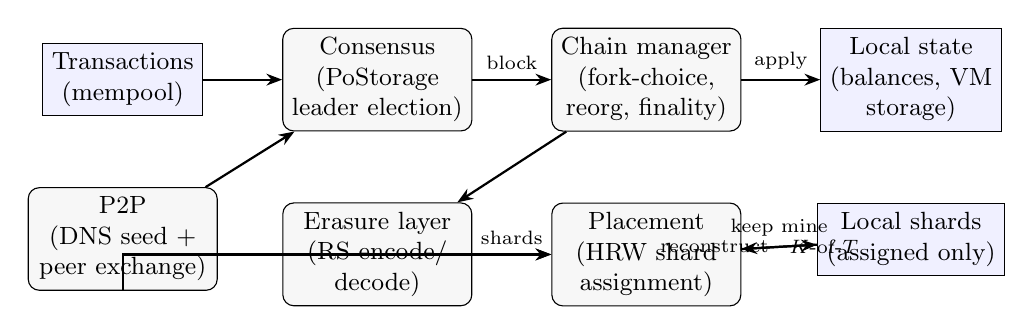
\begin{tikzpicture}[
  font=\small,
  box/.style={draw, rounded corners, minimum height=9mm, minimum width=24mm, align=center, fill=gray!6},
  io/.style={draw, minimum height=8mm, align=center, fill=blue!6},
  arr/.style={-{Stealth[length=2mm]}, thick}]
  \node[io] (tx) {Transactions\\(mempool)};
  \node[box, right=10mm of tx] (cons) {Consensus\\(PoStorage\\leader election)};
  \node[box, right=10mm of cons] (chain) {Chain manager\\(fork-choice,\\reorg, finality)};
  \node[io, right=10mm of chain] (state) {Local state\\(balances, VM\\storage)};
  \node[box, below=9mm of cons] (eras) {Erasure layer\\(RS encode/\\decode)};
  \node[box, below=9mm of chain] (place) {Placement\\(HRW shard\\assignment)};
  \node[io, below=9mm of state] (disk) {Local shards\\(assigned only)};
  \node[box, below=9mm of tx] (p2p) {P2P\\(DNS seed +\\peer exchange)};
  \draw[arr] (tx) -- (cons);
  \draw[arr] (cons) -- node[above,font=\scriptsize]{block} (chain);
  \draw[arr] (chain) -- node[above,font=\scriptsize]{apply} (state);
  \draw[arr] (chain) -- (eras);
  \draw[arr] (eras) -- node[above,font=\scriptsize]{shards} (place);
  \draw[arr] (place) -- node[above,font=\scriptsize]{keep mine} (disk);
  \draw[arr] (p2p) -- (cons);
  \draw[arr] (p2p) |- (place);
  \draw[arr] (disk) -- node[right,font=\scriptsize]{$K$-of-$T$} node[left,font=\scriptsize]{reconstruct} (place);
\end{tikzpicture}
\caption{ShadowLedger node architecture. A leader assembles transactions, the chain manager
applies the state transition (kept local) and hands the body to the erasure layer; HRW placement
keeps only the node's assigned shards and discards the full body. Old bodies are reconstructed on
demand from any $K$-of-$T$ shards gathered over the P2P layer.}
\label{fig:arch}
\end{figure*}

\begin{table}[t]
\centering
\caption{Notation.}
\label{tab:notation}
\small
\begin{tabular}{ll}
\toprule
symbol & meaning \\
\midrule
$n$ & number of live nodes \\
$K,M$ & RS data / parity shards; $T=K{+}M$ \\
$r$ & holders per shard (replication factor) \\
$|b|$ & block body size \\
$f$ & per-node unavailability probability \\
$F$ & finality depth (blocks behind head) \\
$N$ & faucet PoW difficulty (leading zero bits) \\
$\tau$ & target block time \\
\bottomrule
\end{tabular}
\end{table}

A ShadowLedger node runs five cooperating subsystems (Figure~\ref{fig:arch}): (i) an \emph{erasure layer} that encodes
and reconstructs block bodies; (ii) a \emph{placement} module computing HRW shard assignments
from the live membership; (iii) a \emph{consensus engine} (Proof-of-Storage leader election
over the bonded registry); (iv) a \emph{chain manager} holding the fork-choice tree, reorg, and
finality logic plus the local state; and (v) a \emph{peer-to-peer} layer with DNS-seed and
peer-exchange discovery (no central server). The lifecycle of a block is: a leader assembles
transactions, computes the state transition, signs a header committing the body hash and
per-shard hashes, and broadcasts the block; each node applies the state transition, then keeps
only its HRW-assigned shards and discards the full body. Reconstruction is on demand: a node
that needs an old body gathers $K$ shards from current holders and checks them against the
committed hashes.

\textbf{Design goals.} The architecture is shaped by five requirements that the rest of the paper
returns to. \textbf{G1 (storage scarcity):} per-node history cost should shrink as the network
grows, not stay constant (\S\ref{sec:storagemodel}). \textbf{G2 (fast validation):} validating a
new block must not require a network round-trip, so the working set stays local
(\S\ref{sec:history}). \textbf{G3 (permissionless, Sybil-resistant entry):} anyone may join as a
validator, but identities must carry a cost (\S\ref{sec:consensus}). \textbf{G4 (convergence and
irreversibility):} temporary partitions must heal, and sufficiently deep history must become
unchangeable (\S\ref{sec:fork}). \textbf{G5 (capital-free onboarding):} a participant with no
tokens must have a path to acquire a small amount without a trusted faucet operator
(\S\ref{sec:econ}). No single mechanism meets all five; the contribution is their composition.

\section{Erasure-Coded History}
\label{sec:history}
\subsection{State versus history}
The pivotal design decision is to treat \emph{state} and \emph{history} differently.
\emph{State}, account balances, nonces, contract storage, is the materialized result of
replaying history; it is bounded (one entry per active account or storage slot) and every
validator keeps it in full locally, exactly as Bitcoin keeps the UTXO set and Ethereum the
state trie. \emph{History}, the block bodies that produced that state, is unbounded and is
the \emph{only} thing fragmented away. Because state is derivable, losing a node's local copy
is not data loss: it is recomputed by replay, or fetched as a snapshot from a peer and checked
against the committed chain. This separation is precisely what lets ``no node stores all
history'' coexist with fast, deterministic validation: validation reads \emph{state}, which is
local; only audit, sync, and dispute resolution need \emph{history}, which is recoverable.

\subsection{Encoding, placement, reconstruction}
On commit, a block body $b$ of size $|b|$ is RS-encoded into $T=K{+}M$ shards, each of size
$\lceil |b|/K\rceil$ (data shards padded; parity shards equal size). The erasure shape
$(K,M)$ is chosen adaptively from the live node count $n$ (\S\ref{sec:overview}); the leader
stamps it into the signed header, so peers read the shape rather than agreeing on it. Each
shard index $s$ is assigned to the top-$r$ nodes under $\mathrm{HRW}(\textit{blockID},s)$,
where $r$ is a replication factor that also scales with $n$. A node persists only the shards
it wins and discards $b$. The header commits $\mathit{BodyHash}(b)$ and the vector of per-shard
hashes; any node gathering $K$ valid shards reconstructs $b$ and verifies
$\mathit{BodyHash}=\,$commitment, so a lying holder is detected and skipped.

\emph{Concrete walkthrough.} Consider a $128$-node network producing block $1000$ with a $1$\,MiB
body. The shape is K16\,M8, so the body becomes $24$ shards of $64$\,KiB each, and the header
commits one $32$-byte hash per shard plus the body hash. Node $X$ computes
$\mathrm{HRW}(\textit{id}_{1000},s)$ for every shard $s$ and finds it ranks in the top
$r{=}3$ for, say, shards $\{3,7\}$; it stores those two ($128$\,KiB) and discards the
$1$\,MiB body. Months later an auditor requests block $1000$: it queries holders, collects any
$16$ of the $24$ shards (each verified against its committed hash), runs RS decode to rebuild the
$1$\,MiB body, and checks the body hash. If eight holders are offline the remaining sixteen still
suffice; if a malicious holder returns a corrupted shard, its hash mismatch excludes it and another
holder's shard is used instead. Node $X$ never reconstructed the block to validate the chain ahead
of it; it only did so on this explicit audit request.

\begin{figure}[t]
\centering
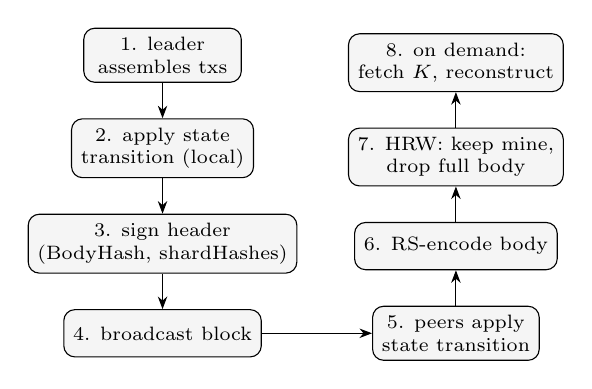
\begin{tikzpicture}[font=\scriptsize, node distance=4.5mm,
  lcell/.style={draw, rounded corners, fill=gray!8, align=center, minimum width=20mm, minimum height=6mm},
  a/.style={-{Stealth[length=1.6mm]}}]
  \node[lcell] (s1) {1. leader\\assembles txs};
  \node[lcell, below=of s1] (s2) {2. apply state\\transition (local)};
  \node[lcell, below=of s2] (s3) {3. sign header\\(BodyHash, shardHashes)};
  \node[lcell, below=of s3] (s4) {4. broadcast block};
  \node[lcell, right=14mm of s4] (s5) {5. peers apply\\state transition};
  \node[lcell, above=of s5] (s6) {6. RS-encode body};
  \node[lcell, above=of s6] (s7) {7. HRW: keep mine,\\drop full body};
  \node[lcell, above=of s7] (s8) {8. on demand:\\fetch $K$, reconstruct};
  \draw[a] (s1)--(s2); \draw[a] (s2)--(s3); \draw[a] (s3)--(s4);
  \draw[a] (s4)--(s5); \draw[a] (s5)--(s6); \draw[a] (s6)--(s7); \draw[a] (s7)--(s8);
\end{tikzpicture}
\caption{Block lifecycle: state is applied and kept by all; the body is encoded, only assigned
shards are retained, and old bodies are reconstructed on demand.}
\label{fig:lifecycle}
\end{figure}

\subsection{Storage model}
\label{sec:storagemodel}
Let each shard have $r$ holders and let the $T$ shards be spread over $n$ nodes by HRW. The
expected number of shard copies a node holds for one block is $Tr/n$, each of size $|b|/K$, so
expected per-node storage per block is
\[
S_{\text{node}} \;=\; \frac{Tr}{n}\cdot\frac{|b|}{K}.
\]
Full replication stores $|b|$ per node, giving a reduction factor
\[
\rho \;=\; \frac{|b|}{S_{\text{node}}} \;=\; \frac{Kn}{Tr}.
\]
With ShadowLedger's policy ($T,K$ saturate at $K{=}16,M{=}8$ and $r{=}3$ for large $n$),
$\rho \approx Kn/(Tr) = 16n/(24\cdot3)=n/4.5$, i.e.\ per-node history cost falls as
$O(1/n)$ while full replication is constant. Below $n\!\approx\!4$ the fixed parity overhead
$T/K$ dominates and fragmentation is not yet a win, an honest small-network regime we report
rather than hide. \S\ref{sec:eval} validates this model empirically against rendezvous
placement.

\subsection{Sync and state snapshots}
\label{sec:sync}
A node that joins late, or that lost its local state, must reach the current head without
necessarily replaying every historical body. Two paths exist. The \emph{header-first} path
downloads the (small, signed) header chain and verifies its links and signatures, giving the node
a trustworthy skeleton of heights, commitments, and the validator set; bodies are then fetched and
reconstructed only as needed (\S\ref{sec:eval} quantifies that cost). The \emph{snapshot} path
fetches a materialized state at a recent height from a peer and adopts it as a \emph{checkpoint}:
the node sets its replay base (\S\ref{sec:fork}) to that height, so it can still reorg above the
checkpoint but trusts the snapshot below it. Because the snapshot is the fold of all prior blocks,
its correctness is in principle checkable by replay; making it succinctly \emph{verifiable}
without replay needs a committed state root, which the present header omits (\S\ref{sec:disc}). In
both paths, steady-state operation then reverts to keeping only HRW-assigned shards: sync cost is
paid once, storage savings persist.

\section{Proof-of-Storage Consensus}
\label{sec:consensus}
\textbf{Bonded validator registry.} Validators are on-chain state, not configuration. A node
joins by submitting a \emph{register} transaction that locks a bond (skin-in-the-game, in the
spirit of PoS deposits~\cite{kiayias2017ouroboros,buterin2017casper}) and solves a one-shot
registration PoW. The PoW is \emph{not} block production: it is a Sybil gate that makes mass
fake identities expensive and seeds shard-assignment randomness, exactly as one-shot PoW is
used for committee formation in Elastico~\cite{luu2016elastico}. The active registry is read
live from state, so registration changes the producer set with no reconfiguration round and
every node derives the same set deterministically.

The two entry costs are complementary. The \emph{bond} is recoverable capital that creates
skin-in-the-game: it is returned on a clean exit but burned on equivocation
(\S\ref{sec:fork},~\ref{sec:threat}), so it deters misbehavior rather than entry. The
\emph{registration PoW} is a one-time sunk compute cost that deters \emph{mass} entry: minting $m$
Sybil identities costs $m$ independent puzzle solutions, making large fake fleets expensive even if
each bond is small. The difficulty is a tunable parameter, set so a single honest registration is
sub-second while a fleet of thousands is costly; \S\ref{sec:eval} reports the analogous cost curve
for the faucet PoW, which uses the same primitive. Because the puzzle is bound to the registering
address, its solution doubles as an unbiased seed for that identity's shard-assignment and
leader-election ranking, so a validator cannot choose which shards or slots it will win.

\textbf{Storage-weighted leader election.} For height $h$ and round $t$, the leader is chosen by
HRW over the active validators seeded by $(\textit{prevHash},h,t)$, but \emph{weighted by proven
storage}: each validator is given $1+\min(\textit{score},C)$ virtual HRW entries, where
$\textit{score}$ is its count of accepted on-chain storage proofs (\S\ref{sec:audit}) and $C$ caps
the bonus. The weight is integer-only, so every node computes the identical election from
deterministic chain state, and a validator that stops proving decays to the base weight of one. The
rank depends on the previous block hash, so it is unpredictable until the parent is fixed and cannot
be ground out in advance (\S\ref{sec:threat}). Block-production odds therefore track demonstrated
storage rather than mere registration.

\textbf{Implementation status (what is built vs.\ specified).} To avoid overclaiming, we separate
the two precisely. \emph{Built and evaluated}: the bonded on-chain registry, the one-shot
registration PoW, the on-chain storage-proof transaction and its verification against committed
shard hashes (\S\ref{sec:audit}), storage-weighted HRW leader election driven by those proofs with
round fallback, equivocation slashing, the reorg engine, and depth-based finality. \emph{Specified
but not yet built}: slashing a validator's \emph{bond} for missed storage proofs (the prototype
applies the softer penalty of election-weight decay, not bond burn) and storage-weighted
\emph{fork choice} (branch weight remains chain length, \S\ref{sec:fork}). The election is genuinely
storage-coupled in the running binary; what is deferred is the harsher economic punishment and the
extension of weighting from leader selection to branch selection.

\textbf{Liveness fallback.} A silent leader must not stall the chain. Round $t$ is derived from
elapsed time since the parent ($t=\lfloor\Delta/\tau\rfloor$ for block time $\tau$); if round-0's
leader produces nothing within one block time, round $1$ elects a \emph{different} validator,
and so on. Headers carry $t$, and a block is rejected unless its timestamp is consistent with
its claimed round ($\textit{ts}\ge \textit{prevTs}+t\tau$), so a high round cannot be claimed
early. Genesis uses a fixed timestamp to anchor the schedule identically on all nodes
(Algorithm~\ref{alg:leader}).

\begin{algorithm}[t]
\SetAlgoLined\DontPrintSemicolon
\KwIn{height $h$, parent header $P$, local time $\textit{now}$, block time $\tau$, my id $\textit{me}$}
$V \leftarrow \textsc{ActiveValidators}()$ \tcp*{live from on-chain registry}
$t \leftarrow \max(0,\lfloor(\textit{now}-P.\textit{ts})/\tau\rfloor)$ \tcp*{elapsed rounds}
$\textit{leader} \leftarrow \arg\max_{v\in V}\ \textsc{HRW}(P.\textit{hash},h,t,v)$\;
\If{$\textit{leader}=\textit{me}$ \textbf{and} have-work}{
  build block at $(h,t)$ with $\textit{ts}\ge P.\textit{ts}+t\tau$; sign; broadcast\;
}
\caption{Proof-of-Storage leader election with round fallback (run each tick).}
\label{alg:leader}
\end{algorithm}

\textbf{Slashing.} Two validly signed, conflicting headers at the same height by one validator
are provable equivocation. A \emph{slash} transaction carries the two headers as evidence; it
burns the offender's bond (a fraction rewards the reporter) and permanently bars the identity,
following Casper/Tendermint practice~\cite{buterin2017casper,buchman2018gossip}.

\section{Storage Auditing}
\label{sec:audit}
Proof-of-Storage is only as strong as the network's ability to \emph{check} that a node holds
what it claims. ShadowLedger runs a lightweight challenge--response audit, in the lineage of
proofs of retrievability~\cite{juels2007pors} and replication~\cite{fisch2018scaling} but
specialized to committed shards.

\textbf{Challenge--response.} Periodically, a node challenges a holder for one of its assigned
shards $(\textit{blockID},s)$ with a fresh random nonce $c$. The holder replies with
$\sigma=H(\textit{shard}\,\|\,c)$. Because the header commits the shard's hash, a challenger can
detect a holder that does not actually possess the bytes: a holder without the shard cannot
produce a $\sigma$ consistent with the committed shard (it would have to invert $H$), and a
holder that serves a \emph{wrong} shard is caught when any reconstructing node compares the
committed hash. The nonce prevents replaying a previously observed response, so the holder must
have the shard \emph{now}, not merely once.

\textbf{Scoreboard.} Each node keeps a local scoreboard of pass/miss outcomes per peer. A peer
that repeatedly fails challenges, or serves shards inconsistent with their commitment, is
down-scored and, for outright forgery, struck from the local peer set. The scoreboard is a fast local
hygiene signal; the consensus-binding counterpart is the on-chain storage score described next,
which \S\ref{sec:consensus} reads so a validator that proves it stores more of its assigned shards
wins more rounds.

\textbf{On-chain storage-proof records.} The audit is made consensus-visible by a storage-proof
transaction. A validator periodically proves it can produce a \emph{protocol-assigned} shard of a
recent confirmed block: the target block lies within a recency window and at least a few blocks
deep, and the shard \emph{index} is derived deterministically as $H(\textit{addr}\,\|\,
\textit{blockID})\bmod T$, so the validator cannot cherry-pick one easy shard but must answer for
the slot the protocol assigns it (it serves the shard locally if it holds it, or reconstructs it
from $K$ peers). Every node verifies the submitted bytes against the committed shard hash for that
slot, taken from the persisted header and shard set, so verification needs neither the full body
nor any new header field. An accepted proof increments the validator's on-chain
\emph{storage score} (capped), which \S\ref{sec:consensus} reads to weight leader election; the
score decays to the base if the validator stops proving within the window.

\textbf{Status and honest scope.} What this buys, in the running binary, is storage-\emph{coupled}
election: block-production odds rise with accepted proofs and fall when proofs lapse, a real
economic pressure to store and serve assigned data. What it does \emph{not} yet do is burn a
validator's \emph{bond} for missed proofs (the penalty is weight decay, softer than a slash) or
weight \emph{fork choice} by storage (branch weight is still chain length, \S\ref{sec:fork}). The
local scoreboard remains as a fast peer-hygiene tool alongside the on-chain record. We separate
these precisely (\S\ref{sec:consensus}, \S\ref{sec:disc}) rather than let the term
``proof-of-storage'' imply more than is enforced.

\section{Fork Choice, Reorganization, and Finality}
\label{sec:fork}
\textbf{Fork choice.} Nodes maintain a block tree and follow the heaviest branch, after
GHOST~\cite{sompolinsky2015ghost}; ties break by lowest block id for determinism. Today
``weight'' is chain length. We deliberately keep this distinct from \emph{leader election}, which
\emph{is} storage-weighted (\S\ref{sec:consensus}). Extending storage weight to branch selection is
not a free relabelling: a branch's weight must be computed identically by every node for any
competing branch, yet a producer's storage score is \emph{branch-dependent state} (it depends on
which proofs that branch accepted). Making fork choice storage-weighted therefore requires either
committing each producer's score in the (signed) header or recomputing weights by replaying each
branch, and a naive local-state reading would let nodes disagree on the heaviest branch, a
consensus-safety hazard. We treat this as future work rather than risk that on a live network; the
leader-election weighting, whose inputs are the post-parent state both producer and verifier already
share, has no such hazard.

\textbf{Reorg engine.} On observing a heavier branch, a node rewinds state to a \emph{replay
base} and replays the winning branch onto a fresh copy, committing only if the whole branch
applies cleanly, so a malformed branch can never corrupt live state. A linear extension of
the current head is fast-forwarded without a full replay.

\textbf{Depth-based finality.} The replay base advances to $\textit{head}-F$ as the chain grows
and never moves backward. Because a reorg can rewind no further than the replay base, a
competing branch that forks \emph{below} the finalized height $\textit{head}-F$ literally cannot
be applied: it cannot reach the base to replay from, and is refused. Thus history older than
$F$ blocks is irreversible. The safety of depth-based finality rests on the common-prefix
property: for an honest-majority bonded set, the probability that an $F$-deep block is later
displaced decays exponentially in $F$~\cite{garay2015backbone}; the prototype sets $F{=}16$
(Algorithm~\ref{alg:final}).

\begin{algorithm}[t]
\SetAlgoLined\DontPrintSemicolon
\KwIn{head $H$, finality depth $F$, replay base $(B,\textit{baseHt})$}
\lIf{$H.\textit{height}-F \le \textit{baseHt}$}{\Return}
$\textit{target} \leftarrow H.\textit{height}-F$\;
walk $H \rightsquigarrow B$, collecting canonical blocks with height $\le \textit{target}$\;
$S \leftarrow \textsc{Clone}(\textit{baseState})$;\ replay collected blocks onto $S$ in order\;
advance replay base to deepest replayed block; persist; \textbf{base never moves back}\;
\tcp{a fork below the base cannot reach it $\Rightarrow$ reorg refused}
\caption{Depth-based finality advance (after the head changes).}
\label{alg:final}
\end{algorithm}

\textbf{Safety and liveness, informally.} Safety of finality reduces to a single invariant: the
replay base is monotone non-decreasing in height. Since every reorg target is reached by walking
down to the replay base and a fork below it cannot be walked to, no committed block at height
$\le \textit{baseHt}$ is ever rewritten. The base advances only to $\textit{head}-F$, so the
window of mutable history is bounded by $F$, and the probability that an honest $F$-deep block is
displaced before finalization decays as the common-prefix bound in
$F$~\cite{garay2015backbone,sompolinsky2015ghost}. Liveness is provided by the round fallback of
\S\ref{sec:consensus}: if the round-$t$ leader is silent, round $t{+}1$ elects a different
validator, so as long as some honest validator is eligible and online the head advances and, with
it, the finalized height. The two properties are independent: the round mechanism guarantees
progress, while the monotone base guarantees that progress, once $F$ deep, is permanent.

\begin{figure}[t]
\centering
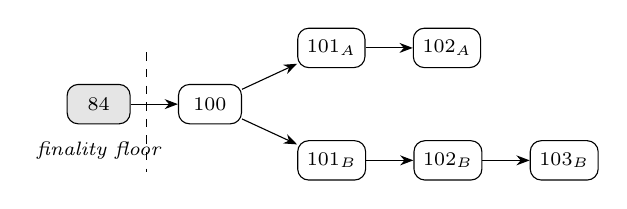
\begin{tikzpicture}[font=\scriptsize, >=Stealth,
  blk/.style={draw, rounded corners, minimum width=8mm, minimum height=5mm},
  fin/.style={draw, rounded corners, minimum width=8mm, minimum height=5mm, fill=gray!20}]
  \node[fin] (b84) {84};
  \node[blk, right=6mm of b84] (b100) {100};
  \node[blk, above right=2mm and 7mm of b100] (a101) {$101_A$};
  \node[blk, right=6mm of a101] (a102) {$102_A$};
  \node[blk, below right=2mm and 7mm of b100] (b101) {$101_B$};
  \node[blk, right=6mm of b101] (b102) {$102_B$};
  \node[blk, right=6mm of b102] (b103) {$103_B$};
  \draw[->] (b84)--(b100);
  \draw[->] (b100)--(a101); \draw[->] (a101)--(a102);
  \draw[->] (b100)--(b101); \draw[->] (b101)--(b102); \draw[->] (b102)--(b103);
  \node[below=1mm of b84, font=\scriptsize\itshape] {finality floor};
  \draw[dashed] ($(b84.north east)+(2mm,4mm)$) -- ($(b84.south east)+(2mm,-6mm)$);
\end{tikzpicture}
\caption{Reorg above the finality floor. Branch $B$ (heavier, height $103$) wins over branch $A$;
nodes rewind to the common parent $100$ and replay $B$. Blocks at or below the floor (height $84$,
shaded) are final and cannot be reorganized.}
\label{fig:reorg}
\end{figure}

\emph{Worked reorg.} Suppose a partition leaves validator $A$ extending tip
$\dots{\to}100{\to}101_A{\to}102_A$ while validator $B$ extends
$\dots{\to}100{\to}101_B{\to}102_B{\to}103_B$ from the same parent at height $100$. When the
partition heals, every node sees both branches; $B$'s is heavier (height $103$ versus $102$), so a
node currently on $A$'s tip walks back to the last common point (height $100$, which is at or above
its replay base), rewinds its state to that point, and replays $101_B,102_B,103_B$ onto a fresh copy.
It commits only after all three apply cleanly, then adopts $103_B$ as head; nodes already on $B$
simply keep it. If instead $B$'s branch had forked at height $80$ while the replay base had already
advanced to $84$ (finality depth reached), the walk-back could not reach a replayable base and the
reorg would be refused outright, since heights $\le 84$ are final. Convergence above the finality
floor, immutability below it.

\section{Economics and Capital-Free Onboarding}
\label{sec:econ}
\textbf{Issuance.} The native unit \$SHARD\ follows a Bitcoin-style schedule: a fixed maximum
supply and a block subsidy that halves every fixed number of blocks, paid to the block's validator
as a coinbase together with the transaction fees of that block. Two invariants keep the schedule
deterministic and non-inflationary. First, only the subsidy counts against the cap; fees are
recycled from payers to the producer, never newly minted, so total issuance is exactly the sum of
the (geometrically decaying) subsidies and is bounded by the cap. Second, the faucet pays from a
pre-funded treasury balance rather than minting, so onboarding grants do not perturb the schedule.
A node validates the coinbase against the schedule on every block, rejecting any block whose
coinbase exceeds the height's allowed subsidy plus its fees, so a producer cannot pay itself more
than the protocol permits.

\textbf{PoW faucet.} A brand-new follower holds no \$SHARD\ and can pay neither fees nor a bond.
The faucet is the on-ramp: the follower mines a nonce so that
$H(\textit{chainID}\,\|\,\textit{addr}\,\|\,\textit{anchorBodyHash}\,\|\,\textit{nonce})$ has $N$
leading zero bits, and claims a small fixed payout drawn from the treasury (\emph{not} newly
minted, so the cap is untouched). The anchor is a recent block's committed body
hash, present in the signed header, hence verifiable by \emph{every} node without holding the
fragmented body, the same data-availability-safe principle as the rest of the design. The anchor
is unknown until the block exists, so claims cannot be precomputed; a per-address cooldown and
the tunable hashing cost rate-limit abuse, giving a Sybil price linear in the number of
identities (Algorithm~\ref{alg:faucet}).

\begin{algorithm}[t]
\SetAlgoLined\DontPrintSemicolon
\KwIn{claim tx from $a$ at height $h$: (anchorHt, nonce); params $N,F_{\!f},\textit{cool},\textit{amt}$}
\lIf{$\textit{anchorHt}+F_{\!f}>h$ \textbf{or} $h-\textit{anchorHt}>256$}{reject \tcp*{unconfirmed/stale}}
$\textit{anchor} \leftarrow \textsc{HeaderBodyHash}(\textit{anchorHt})$ \tcp*{from signed header; no body needed}
\lIf{$\textsc{Lz}(H(\textit{chainID}\|a\|\textit{anchor}\|\textit{nonce}))<N$}{reject \tcp*{bad PoW}}
\lIf{$h<\textit{lastClaim}[a]+\textit{cool}$}{reject \tcp*{cooldown}}
treasury $\!-\!=\textit{amt}$;\ balance$[a]\!+\!=\textit{amt}$;\ $\textit{lastClaim}[a]\leftarrow h$\;
\caption{Faucet claim verification (\textsc{Lz}: leading-zero-bit count).}
\label{alg:faucet}
\end{algorithm}

\section{Deterministic Smart Contracts}
\label{sec:vm}
We treat programmability as a \emph{supporting capability}, not a scientific contribution of this
paper: the core results concern fragmented history and the storage-coupled consensus, and a reader
interested only in those may skip this section. We include it because a storage-scarce ledger is of
little use if it cannot run application logic, and because the contract layer must obey the same
commitment discipline (signed roots, deterministic execution) as the rest of the system; we
therefore keep the description brief.

Contracts execute on a deterministic stack virtual machine with metered gas. Determinism is a hard
requirement: every node that runs the same bytecode on the same input and storage must reach the
same result, or consensus over contract state breaks. The VM therefore excludes every source of
nondeterminism, namely wall-clock time, floating point, and randomness, and bounds execution by a
gas budget and a step limit so a contract cannot loop forever or exhaust memory.

\textbf{Machine model.} The VM is a stack machine over $64$-bit words with a per-contract
key/value store (uint64 to uint64). Opcodes fall into the classes of Table~\ref{tab:opcodes}.
Storage writes are the expensive operation, reflecting their real cost (they enlarge the state
every node keeps), so gas pricing discourages gratuitous writes. Cross-contract calls are allowed
but bounded by a call-depth limit, which caps reentrancy and recursion. Because a $64$-bit word
cannot hold a $20$-byte address or a string, a byte-storage layer holds variable-length blobs
(addresses, token identifiers, URIs) sourced from calldata, with opcodes to store, compare, hash,
and return them; this is how a contract can manipulate full addresses despite the uint64 core.

\begin{table}[t]
\centering
\caption{VM opcode classes (representative, not exhaustive).}
\label{tab:opcodes}
\small
\begin{tabular}{ll}
\toprule
class & opcodes / role \\
\midrule
arithmetic    & add/sub/mul (overflow-checked), div/mod (revert on $0$) \\
logic/compare & and, or, not, eq, lt, gt, iszero \\
stack         & push, pop, dup, swap \\
control flow  & jump, jumpi, stop, return, revert \\
storage       & sload, sstore, mix (mapping-slot hash) \\
environment   & caller, value, self, calldata, calldata-len \\
byte layer    & bstore, beq, bhash, caller-bytes, return-bytes \\
events / calls& log (committed in LogsRoot), call (depth-bounded) \\
\bottomrule
\end{tabular}
\end{table}

\textbf{The SHL language.} Writing raw bytecode is error-prone, so contracts are written in SHL, a
small Solidity-like language compiled through a lexer, parser, and code generator. SHL offers named
\texttt{state} variables and mappings (each assigned a fixed storage slot by the compiler, so there
are no hand-managed magic offsets), functions with selector dispatch, \texttt{require} and
\texttt{revert} with full state rollback, and overflow-checked arithmetic by default. A function
selector is derived from the function name and placed in the call's first calldata word; the
compiler emits a dispatcher that routes to the matching function and reverts on an unknown selector.
Listing~\ref{lst:shl} shows a fungible-token transfer: the \texttt{require} guard reverts the entire
call (restoring all storage) if the sender is short, and both updates are overflow-checked, so a
short and readable contract is also a safe one.

\begin{lstlisting}[caption={A safe ERC-20-style transfer in SHL.},label={lst:shl}]
state balances;          // mapping holder -> amount
state totalSupply;

fn transfer(to, amount) {
  require(balances[msg.sender] >= amount);
  balances[msg.sender] = balances[msg.sender] - amount; // checked
  balances[to] = balances[to] + amount;                 // checked
  emit(TRANSFER, msg.sender, to, amount);
}
fn balanceOf(who) { return balances[who]; }
\end{lstlisting}

\textbf{Scope.} SHL is deliberately a faithful \emph{subset} of the Solidity model rather than a
clone. It omits $256$-bit integers, contract inheritance, and the ABI, trading generality for a VM
small enough to audit and reason about, which suits a system that has not yet undergone external
security review (\S\ref{sec:disc}). Events emitted via \texttt{log} are committed through the block
header's logs root, so a verifier can later prove that an event occurred without trusting the node
that serves it, the same commitment discipline used for shards and transactions.

\section{Threat Model and Security Analysis}
\label{sec:threat}
We assume an adversary that can run nodes, register as a validator (paying bond + PoW), send
arbitrary messages, and partition the network temporarily, but cannot break ed25519 signatures
or SHA-256, and does not control a majority of the bonded stake.

\textbf{Block injection / poisoning.} Every header field is signed and validated; each shard is
committed by hash. An outsider cannot insert a block: forged signatures, unauthorized producers,
tampered bodies (Merkle/body-hash mismatch), wrong height or parent, future timestamps, and
forged log roots are all rejected (\S\ref{sec:eval} exercises seven such variants). A lying shard
server is detected by the committed shard hash and skipped.

\textbf{Data withholding.} A producer could publish a header but withhold body shards. The
availability-first canonical rule treats a block that cannot be reconstructed to its commitment
as not-yet-valid; reconstruction succeeds as long as $K$ honest holders exist, which the
replication factor $r$ and HRW spread are sized to ensure. Succinct DA
sampling~\cite{hallandersen2025foundations} would strengthen this from an operational check to a
probabilistic proof and is future work.

\textbf{Availability analysis.} Quantify recoverability under random node loss. If each node is
independently unavailable with probability $f$ and a shard has $r$ holders, that shard is lost
only if all its holders are down, w.p.\ $f^r$, so it is available w.p.\ $p=1-f^r$. A block of $T$
shards is recoverable iff at least $K$ shards survive:
\[
\Pr[\text{recoverable}] \;=\; \sum_{i=K}^{T}\binom{T}{i}p^{\,i}(1-p)^{\,T-i}.
\]
Table~\ref{tab:avail} evaluates this for the saturated shape (K16\,M8, $r{=}3$). A shard is lost
only when all three independently chosen holders are simultaneously down ($f^3$), and the code
still tolerates $M{=}8$ such losses; the block-loss probability is therefore dominated by
$\binom{T}{M+1}(f^3)^{M+1}$ and is negligible even at a severe $f{=}0.3$. This is the quantitative
reason fragmentation does not trade away durability: replication ($r$) protects each shard, and
parity ($M$) protects the block.

\begin{table}[t]
\centering
\caption{Recoverability at K16\,M8, $r{=}3$, $T{=}24$. Shard loss $f^3$; block lost iff $>M$ shards lost.}
\label{tab:avail}
\small
\begin{tabular}{rrr}
\toprule
$f$ & shard-loss $f^3$ & $\Pr[\text{block lost}]$ (bound) \\
\midrule
0.05 & $1.3\times10^{-4}$ & $<10^{-30}$ \\
0.10 & $1.0\times10^{-3}$ & $<10^{-20}$ \\
0.20 & $8.0\times10^{-3}$ & $<10^{-11}$ \\
0.30 & $2.7\times10^{-2}$ & $<10^{-6}$ \\
\bottomrule
\end{tabular}
\end{table}

\textbf{Correlated and colluding holders.} The durability argument above assumes node failures are
\emph{independent}; the $f^r$ term is exactly this assumption. It is the model's main soft spot.
If the $r$ holders of a shard are correlated (same operator, same data center, or a storage pool
under one administrator), losing or withholding that shard costs far less than $f^r$ suggests, and
a colluding set that holds all $r$ copies of enough shards can selectively withhold a block while
appearing online. HRW placement spreads holders by identity, not by operator, so it does not by
itself defeat an adversary who registers many identities behind one back end (the registration PoW
raises but does not eliminate that cost). Two defenses are partial today and strengthen with the
specified work: replication $r$ and parity $M$ raise the number of distinct holders that must
collude, and the storage-weighted election (built) plus future bond slashing for missed proofs make
holding-but-withholding economically self-defeating. We state this as a real limitation, not a solved problem.

\textbf{Sybil and long-range attacks.} Mass identities cost bond + registration PoW per
identity. Rewriting finalized history is impossible by construction (\S\ref{sec:fork}); a
heavier-but-late branch below the finality depth is refused. Above the finality depth, the
heaviest honest branch wins.

\textbf{Leader grinding.} Because leader election is
$\mathrm{HRW}(\textit{prevHash},h,t)$, an adversary might try to bias future elections by choosing
the content of a block it produces so that the resulting hash favors its own future rank. Two
factors limit this. First, the registration PoW seeds each identity's HRW key, so an attacker
cannot cheaply mint identities whose keys win specific slots. Second, influencing $\textit{prevHash}$
requires actually producing the parent block (already a won election) and only shifts the
\emph{next} slot probabilistically, not deterministically; grinding over many candidate blocks costs
hashing for a marginal bias. The storage-weighted election (\S\ref{sec:consensus}) further binds
odds to a quantity, proven storage, that an attacker cannot grind by reshaping a block: it must
actually answer storage-proof challenges to gain weight.

\textbf{Bond economics.} The bond must exceed the expected gain from misbehavior for slashing to
deter it. Registration requires a minimum bond, and the slash burns it while rewarding the reporter
a fraction, so an equivocating validator faces a certain loss against an uncertain gain. Setting the
minimum bond and slash fraction relative to block reward is a parameter-tuning question we leave to
deployment; the mechanism, not the specific values, is the contribution.

\textbf{Equivocation.} Double-signing is slashable with on-chain evidence, making it
economically irrational. \textbf{Eclipse/networking} attacks are out of scope for this paper and
mitigated only partially (peer diversity); we note them as a limitation. Table~\ref{tab:threat}
summarizes the model.

\begin{table}[t]
\centering
\caption{Threat model summary. \checkmark\,= mitigated in the prototype; $\circ$\,= partial.}
\label{tab:threat}
\small
\begin{tabular}{lll}
\toprule
Threat & Mechanism & Status \\
\midrule
Block injection      & signed header + per-shard hash      & \checkmark \\
Tampered body        & Merkle/body-hash commitment         & \checkmark \\
Lying shard server   & committed shard hash, skip+ban      & \checkmark \\
Data withholding     & availability-first canonical rule   & $\circ$ \\
Sybil identities     & bond + one-shot registration PoW    & \checkmark \\
Equivocation         & slashing with on-chain evidence     & \checkmark \\
Long-range rewrite   & depth-based finality ($F$ deep)     & \checkmark \\
Cross-network replay & chain-id bound into every tx        & \checkmark \\
Eclipse / routing    & peer diversity only                 & $\circ$ \\
\bottomrule
\end{tabular}
\end{table}

\section{Implementation}
\label{sec:impl}
ShadowLedger is implemented in Go as a set of small, independently tested packages: erasure
coding (over an RS library), rendezvous placement, the Proof-of-Storage engine, the chain
manager (fork-choice tree, reorg, finality, state), the uint64 VM and the SHL compiler, the
registration-PoW and faucet-PoW primitives, and the peer-to-peer layer. The network is deployed
as a live prototype with a bootstrap node on a public cloud host plus additional peers;
discovery uses DNS seeds and peer exchange with no central coordinator. The deterministic core
is exercised by an automated test suite spanning roughly sixteen packages. Table~\ref{tab:modules}
lists the principal modules and their responsibilities; the separation keeps each mechanism
independently testable, which is how the security and functional checks of \S\ref{sec:eval} are
obtained in isolation before integration.

\begin{table}[t]
\centering
\caption{Principal implementation modules and responsibilities.}
\label{tab:modules}
\small
\begin{tabular}{ll}
\toprule
module & responsibility \\
\midrule
erasure      & RS encode/decode, shard hashing, reconstruction \\
placement    & HRW shard assignment, holder selection \\
consensus    & Proof-of-Storage leader election, round fallback \\
chain        & fork-choice tree, reorg, finality, block apply \\
state        & accounts, validator registry, contract storage \\
vm + shl     & uint64 VM, gas metering, SHL compiler \\
regpow       & one-shot registration PoW (Sybil gate) \\
faucet       & onboarding PoW, anchor verification \\
p2p          & DNS-seed/peer-exchange discovery, gossip, sync \\
\bottomrule
\end{tabular}
\end{table}

\textbf{Networking and discovery.} Membership is maintained without any central directory. A new
node bootstraps from a small set of DNS seeds baked into the binary, then learns further peers by
exchange (each peer shares a sample of its own peer set), so the view of membership grows and heals
under churn, which is the same set the placement module feeds to HRW. Two channels carry traffic: a
control channel gossips headers and full blocks for state application, and a shard-transfer channel
serves and requests individual shards for reconstruction. Genesis is derived deterministically from
the embedded parameters rather than gossiped, so every node that ships the same binary computes an
identical block~$0$ and therefore an identical chain of prev-hash links, which is what lets a
zero-configuration node join a running network safely.

\textbf{Deployment notes.} The prototype runs as zero-configuration mainnet: network parameters
(genesis, seed nodes, erasure policy) are baked into the binary, so a freshly installed node joins
automatically, in the spirit of how reference clients ship their genesis and seeds. The bootstrap
node runs on a single small cloud instance behind a standard firewall; the only operational
prerequisite is opening the control/transfer ports. Software updates are \emph{advisory}: a node
reports a newer release but never auto-applies it, since silent auto-update would be a central
kill switch in a system whose point is decentralization. We treat the live network as a testnet:
the tokens carry no real value, which lets us exercise consensus, reorg, finality, the faucet, and
contract deployment on a genuinely public deployment without inviting financial risk before an
external audit.

\section{Evaluation}
\label{sec:eval}
\textbf{Methodology.} We report \emph{prototype} measurements, one cloud deployment plus a
developer workstation, as evidence of feasibility, not statistical generalization
(this is a Level-5 systems-design evaluation: an artifact exercised under controlled
conditions). Erasure and placement experiments invoke the production encoder and HRW code paths
directly rather than a re-implementation; storage figures average rendezvous placement of every
shard over $2000$ synthetic blocks per network size; throughput is the mean of $20$ encode/decode
repetitions per body size on a single core; PoW figures are medians over nine independently
generated identities to capture the geometric-distribution variance of the search. Functional and
security results come from the automated test suite and from exercising the live deployment.

\textbf{Reproducibility.} Every measurement here derives from a deterministic code path. The storage
figures are a function of $(n,K,M,r)$ and the rendezvous hash of fixed synthetic block identifiers,
so they reproduce exactly given the same parameters; the throughput numbers depend only on body size
and the single-core encoder; the PoW costs follow the geometric distribution of a fixed difficulty,
which is why we report medians over independent identities rather than a single run. The functional
and security checks are encoded as repeatable tests over the same deterministic core that runs in
production, so a reviewer with the artifact can re-derive each result without access to our specific
cloud host. We consider this the appropriate reproducibility bar for a single-team prototype, short
of the controlled multi-system benchmark we leave to future work (\S\ref{sec:disc}).

\subsection{Storage scarcity}
We instantiate the model of \S\ref{sec:storagemodel} with $1$\,MiB block bodies, the network's
adaptive $(K,M)$ and $r$, and rendezvous placement of every shard over $n$ nodes, averaged over
$2000$ blocks. Table~\ref{tab:storage} reports the bytes each node retains per block and the
reduction versus full replication. The measured reduction tracks the analytical $\rho=Kn/(Tr)$:
per-node history falls roughly as $O(1/n)$ while full replication stays at $1$\,MiB/block/node,
reaching $\approx 28\times$ at $n{=}128$ and widening thereafter. Below $n{=}4$ fragmentation is
not yet a win, as the model predicts.

\begin{table}[t]
\centering
\caption{Per-node history storage vs.\ full replication (1\,MiB blocks; rendezvous placement
averaged over 2000 blocks). ``max'' shards/node stayed within $3\%$ of the mean, confirming HRW
balance.}
\label{tab:storage}
\begin{tabular}{rlrrr}
\toprule
$n$ & spec & $r$ & store/node/blk & reduction $\rho$ \\
\midrule
4   & K3\,M1  & 2 & 683\,KiB & 1.5$\times$ \\
8   & K6\,M2  & 3 & 512\,KiB & 2.0$\times$ \\
16  & K11\,M5 & 3 & 279\,KiB & 3.7$\times$ \\
32  & K16\,M8 & 3 & 144\,KiB & 7.1$\times$ \\
64  & K16\,M8 & 3 & 72\,KiB  & 14.2$\times$ \\
128 & K16\,M8 & 3 & 36\,KiB  & 28.4$\times$ \\
256 & K16\,M8 & 3 & 18\,KiB  & 56.9$\times$ \\
\bottomrule
\end{tabular}
\end{table}

\begin{figure}[t]
\centering
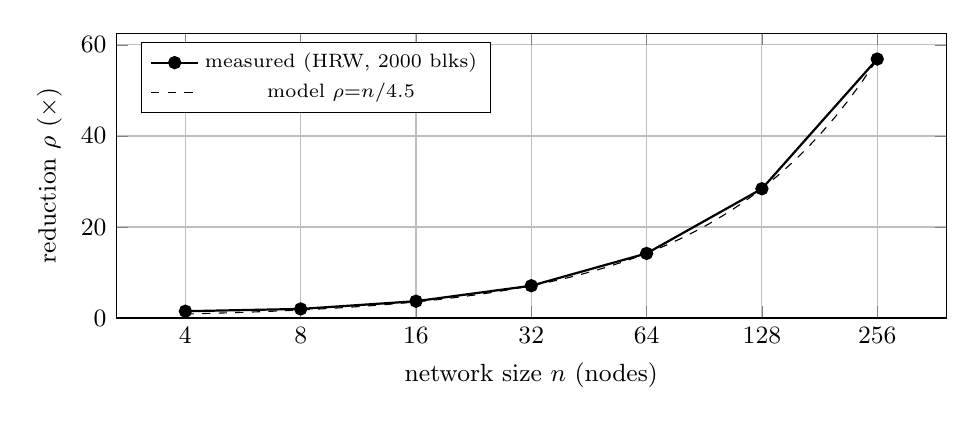
\begin{tikzpicture}
\begin{axis}[
  width=\columnwidth, height=5.2cm, font=\small,
  xlabel={network size $n$ (nodes)}, ylabel={reduction $\rho$ ($\times$)},
  xmode=log, log basis x=2, xtick={4,8,16,32,64,128,256},
  xticklabels={4,8,16,32,64,128,256},
  ymin=0, grid=both, legend pos=north west, legend style={font=\scriptsize}]
\addplot[mark=*,thick] coordinates {(4,1.5)(8,2.0)(16,3.7)(32,7.1)(64,14.2)(128,28.4)(256,56.9)};
\addlegendentry{measured (HRW, 2000 blks)}
\addplot[dashed,domain=4:256,samples=50] {x/4.5};
\addlegendentry{model $\rho{=}n/4.5$}
\end{axis}
\end{tikzpicture}
\caption{Per-node history-storage reduction vs.\ full replication. Measured rendezvous placement
tracks the analytical $\rho=Kn/(Tr)$ once the erasure shape saturates ($n\gtrsim32$).}
\label{fig:storagecurve}
\end{figure}

\subsection{Comparison with replication baselines}
Storage alone is an incomplete metric; the right comparison holds \emph{durability} fixed or
reports both. Table~\ref{tab:baseline} contrasts three schemes for a $128$-node network and
$1$\,MiB blocks: a classic full node (one whole replica per node), naive $3\times$ whole-block
replication distributed over the network, and ShadowLedger (K16\,M8, $r{=}3$). Whole-block
$3\times$ replication is actually \emph{cheaper} per node ($24$\,KiB) than ShadowLedger
($36$\,KiB), but it loses a block whenever the three holders of that block are all down
($\Pr=f^3\approx2.7\times10^{-2}$ at $f{=}0.3$), because there is no parity to recover from a
partial set. ShadowLedger spends $50\%$ more bytes to add erasure parity, buying roughly four
orders of magnitude better durability ($\Pr[\text{loss}]<10^{-6}$ at the same $f$,
\S\ref{sec:threat}) while still storing $\approx28\times$ less than a full node. The adaptive
shape also keeps the data/parity ratio constant as $n$ grows, so the durability margin does not
erode with scale.

\begin{table}[t]
\centering
\caption{Storage vs.\ durability at $n{=}128$, $1$\,MiB blocks, $f{=}0.3$ node unavailability.}
\label{tab:baseline}
\small
\begin{tabular}{lrl}
\toprule
scheme & store/node & $\Pr[\text{block lost}]$ \\
\midrule
full replica (classic node)   & 1024\,KiB & $\approx 0$ (all hold all) \\
$3\times$ whole-block repl.    & 24\,KiB   & $\approx 2.7\times10^{-2}$ \\
\textbf{ShadowLedger} (K16\,M8,$r3$) & 36\,KiB & $<10^{-6}$ \\
\bottomrule
\end{tabular}
\end{table}

\subsection{Coding cost and recoverability}
At the large-network shape (K16\,M8) the coding overhead is fixed at $1.5\times$ ($50\%$ parity).
RS encoding sustains $0.3$--$1.4$\,GB/s and reconstruction from exactly $K$ shards
$0.17$--$0.47$\,GB/s on one core for $64$\,KiB--$4$\,MiB bodies, far above what a $5$\,s block
interval requires, so coding is not a throughput bottleneck. We confirm the all-or-nothing
threshold operationally: with exactly $K$ shards the body is recovered and matches its
commitment; with $K{-}1$ shards reconstruction fails (\emph{not enough shards}) and yields
nothing.

\subsection{Onboarding cost}
Table~\ref{tab:pow} reports faucet-claim cost by difficulty at $\approx 2.5\times10^{6}$
hashes/s on one core. Cost grows geometrically ($+2$ bits $\approx \times4$), a tunable Sybil
price; the deployed difficulty $N{=}18$ costs $\approx 2.6\times10^{5}$ hashes ($\sim$0.1\,s),
cheap for a genuine newcomer yet linear-in-identities for an attacker.

\begin{table}[t]
\centering
\caption{Faucet Proof-of-Work cost by difficulty $N$ (leading zero bits).}
\label{tab:pow}
\begin{tabular}{rrr}
\toprule
$N$ & median hashes & median time \\
\midrule
12 & $3.1\times10^{3}$ & 3\,ms \\
14 & $7.8\times10^{3}$ & 5\,ms \\
16 & $1.5\times10^{5}$ & 65\,ms \\
18 & $2.7\times10^{5}$ & 105\,ms \\
20 & $5.7\times10^{5}$ & 267\,ms \\
\bottomrule
\end{tabular}
\end{table}

\subsection{Parameter sensitivity}
The behaviour above is governed by four knobs: data shards $K$, parity $M$, holders $r$, and
finality depth $F$. Their effects are separable. Per-node storage scales as
$S_{\text{node}}\propto (K{+}M)\,r/(K\,n)$, so it grows with the parity ratio $M/K$ and with $r$,
and shrinks with $n$; the reduction $\rho=Kn/(Tr)$ is what Table~\ref{tab:storage} traces. Durability
is governed by $M$ and $r$ jointly: $r$ sets how hard a single shard is to lose ($f^r$), and $M$
sets how many shard losses the block survives, so the block-loss bound
$\binom{T}{M+1}(f^{r})^{M+1}$ falls steeply in both. Latency of audit/reconstruction depends on $K$
(more data shards means more fetches to gather), and finality latency is exactly $F$ block times.
The policy's saturation at $K{=}16,M{=}8,r{=}3$ is the resulting compromise: a $50\%$ parity ratio
and triple holding keep the loss bound below $10^{-6}$ at $f{=}0.3$ (Table~\ref{tab:avail}) while
capping per-block shard count so coordination and per-shard overhead stay bounded as $n$ grows; $F$
is set so the mutable window (tens of seconds at a $5$\,s interval) is short for users yet ample for
honest reconvergence. These are deployment choices, not fixed constants: a network that values
durability over storage can raise $M$ or $r$, paying the predictable storage cost above.

\subsection{Cost of reconstruction (the tradeoff)}
Fragmentation is not free: a full replica can read any historical body locally, whereas a
ShadowLedger node must gather $K$ shards, about $K\cdot(|b|/K)=|b|$ bytes of network
transfer, to reconstruct one. Reading is thus a bandwidth/latency cost paid only on
\emph{audit, dispute, or sync}, not on normal validation (which touches state, \S\ref{sec:history}).
A late joiner syncing $H$ historical blocks transfers $\Theta(H\,|b|)$ in the worst case of
reconstructing every body, the same asymptotic volume a full replica downloads once; the
difference is that the ShadowLedger node then \emph{discards} all but its assigned shards, so its
\emph{steady-state} footprint is the $O(1/n)$ of Table~\ref{tab:storage} rather than the full
archive. This storage-for-bandwidth trade is the expected shape for coded
blockchains~\cite{kadhe2019sef,perard2018erasure}; ShadowLedger inherits it and confines the cost
to infrequent operations.

\subsection{Consensus behaviour}
We exercised consensus in three regimes. With a single bootstrap validator the chain produces
blocks at the target interval whenever there is work or a subsidy to mint, and idles otherwise,
confirming the round-0 leader path. With a second validator joining via bonded registration, the
HRW rotation alternates producers across heights without any reconfiguration round, since both
derive the active set from identical on-chain state. Under an induced partition, two validators
each extending their own tip, reconvergence occurs as soon as the heavier branch is observed:
the lighter-tip node rewinds to its replay base and replays the winner, ending on the same head
and state (verified by comparing post-reorg balances). Finally, holding a validator silent past
one block time advances the round and lets a different validator produce, demonstrating the
liveness fallback rather than a stall. These are qualitative confirmations on a small validator
set, not a throughput benchmark; large-scale latency/throughput measurement is future work
(\S\ref{sec:disc}).

\emph{Storage-weighted election.} We verify the weighting is effective and deterministic: with two
validators weighted $65{:}1$ by proven storage, the high-storage validator wins $>90\%$ of $2000$
elections while the base-weight validator still wins occasionally, matching the virtual-copy model
of \S\ref{sec:consensus}; every node computes the identical winner from the same chain state. On the public
deployment we observe the loop end-to-end: the validator's auto-submitted storage proofs
(\S\ref{sec:audit}) for protocol-assigned shards are accepted on-chain and its on-chain storage
score rises (e.g.\ to several within the first minutes after the upgrade, visible in the validator
registry), which the election weighting then reads. Block-production odds therefore track proven
storage in the running system, not only in design or in unit tests.

\subsection{Functional and security checks}
\begin{itemize}
  \item \textbf{End-to-end.} The deployed network produced and validated several thousand
  blocks at a $5$\,s target interval; the automated test suite passes across $\sim$16 packages.
  \item \textbf{Tamper resistance.} Seven forged-block variants (\S\ref{sec:threat}) are all
  rejected; an outsider cannot inject a block.
  \item \textbf{Convergence and finality.} Two validators partitioned and re-merged reconverge
  via rewind-and-replay; a reorg below $F{=}16$ is refused by construction.
  \item \textbf{Capital-free onboarding and contracts.} A zero-balance wallet earned its first
  tokens on the live network via the faucet; a fungible-token contract written in SHL was
  deployed and exercised (deploy, initialize, transfer, query) on the live network.
\end{itemize}

\section{Discussion and Limitations}
\label{sec:disc}
We report these candidly, per ACM/COPE integrity expectations. (1) \textbf{Storage coupling, built
and remaining.} Leader election is now storage-weighted via on-chain storage-proof records
(\S\ref{sec:consensus},~\ref{sec:audit}): the running consensus is genuinely storage-coupled. Two
related items remain. \emph{Fork-choice} weight is still chain length (we weight \emph{who leads},
not yet \emph{which branch wins}), and missed storage proofs incur election-weight decay rather than
a \emph{bond} slash. Adding storage weight to fork choice and bond slashing for missed proofs are
the priority next steps and would close the gap between the leader-level and branch-level coupling. (2) \textbf{State commitments}: the header
commits transaction and log roots but not a \emph{state root}, so light clients trust state via
replay/snapshot rather than a succinct proof; adding a state (or verkle) root would enable
trust-minimized light clients~\cite{bunz2020flyclient}. (3) \textbf{Data availability} is an
operational reconstruction check, not a sampling proof; DAS~\cite{hallandersen2025foundations}
is complementary. (4) \textbf{Evaluation scale}: a single deployment and workstation, not a
large multi-region benchmark; numbers are feasibility evidence. (5) \textbf{No external security
audit}; the live network is treated as a testnet with no real value. (6) The contract VM is a
Solidity subset. None of these undermines the central result, that history can be fragmented so
no node stores it all, while state stays local and block production is earned by storage, but
each bounds how far the present prototype should be trusted.

\textbf{Applicability.} ShadowLedger is a fit when history grows large relative to active state and
many modest nodes are available to share it: public ledgers, audit logs, and data-preservation
chains, where the archive dwarfs the working set and decentralization is valued over raw
throughput. It is a poor fit when the working state itself is enormous (then keeping state local is
the bottleneck, and state sharding as in OmniLedger~\cite{kokoriskogias2018omniledger} or
RapidChain~\cite{zamani2018rapidchain} is the right tool), or when historical reads are frequent
and latency-critical (the reconstruction cost of \S\ref{sec:eval} would dominate). The design also
assumes enough independent nodes that the $r$ holders of a shard fail independently; in a tiny or
collusive network that assumption, and with it the availability argument of \S\ref{sec:threat},
weakens. We therefore present ShadowLedger as a point in the design space, not a universal
replacement for replicated ledgers.

\textbf{On head-to-head benchmarking.} We deliberately do not report wall-clock comparisons against
deployed systems such as Filecoin, Chia, or other coded-blockchain prototypes. Such numbers would
be measured on different hardware, networks, and workloads, so a cross-system performance table
would be apples-to-oranges and, by our own integrity standard, misleading; reproducing each system
in a controlled common testbed is a substantial effort beyond this paper. Instead we compare where
comparison is fair: analytically and under identical assumptions against full replication and naive
distributed replication (\S\ref{sec:eval}), and qualitatively against prior coded-storage designs
(\S\ref{sec:related}). The distinction worth stating plainly is not a larger constant-factor saving
than prior coded nodes, which report substantial per-node reductions at a \emph{fixed} network size;
it is that ShadowLedger's reduction \emph{scales} as $O(1/n)$ with the membership and is produced by
the same mechanism that grants block-production rights, rather than by a storage layer bolted onto an
unchanged consensus. A controlled multi-system benchmark on shared infrastructure is the natural next
empirical step.

\section{Design Rationale}
\label{sec:rationale}
Several choices warrant justification beyond their mechanics.

\textbf{Why fragment history but not state?} A naive ``shard everything'' design would force a
network round-trip to read any balance during block validation, making validation latency
non-deterministic and consensus fragile. By keeping the bounded, derivable \emph{state} local and
fragmenting only the unbounded \emph{history}, validation stays a local, deterministic memory
operation while the cost that actually grows without bound is the one distributed
(\S\ref{sec:history}). This mirrors how Bitcoin and Ethereum already keep a working set (UTXO
set / state trie) locally, ShadowLedger simply removes the obligation to also keep the
\emph{archive} locally.

\textbf{Why HRW rather than consistent hashing?} Shard placement must rebalance gracefully as the
permissionless validator set churns. HRW's per-key independent ranking moves only the shards a
joining/leaving node would win/lose, whereas ring-based schemes can shift unrelated
keys~\cite{thaler1998rendezvous,karger1997consistent}. Reusing the same primitive for leader
election keeps the trusted-randomness surface small.

\textbf{Why PoW only as a gate?} Energy-as-security is the property we set out to remove. Yet a
permissionless system still needs a per-identity cost (Sybil resistance) and an onboarding ramp
for the capital-less. Confining PoW to a one-shot registration gate and a small faucet preserves
those properties at negligible aggregate energy, while block ordering, the high-frequency
operation, burns nothing. This is the Elastico insight~\cite{luu2016elastico} applied to a
storage-centric, rather than throughput-centric, design.

\textbf{Why depth-based finality first?} A full finality gadget (e.g.\ Casper
FFG~\cite{buterin2017casper}) adds voting rounds and messages. Depth-based finality reuses the
reorg machinery already needed for fork choice: making the replay base monotone is sufficient to
render deep history irreversible, with safety inherited from the common-prefix
theorem~\cite{garay2015backbone}. It is the smallest change that yields hard irreversibility, and
it composes with a future voting gadget.

\section{Conclusion}
\label{sec:concl}
ShadowLedger reframes the scarce resource of a blockchain from computation to storage. With a
running prototype we show that a chain can fragment its \emph{history} across the
network, so no node stores it all, while keeping \emph{state} local for fast validation,
earning block-production rights by storage-weighted election instead of PoW, and remaining
permissionless through bonded registration and a PoW faucet. An analytical model and measurements
show per-node history cost falling as $O(1/n)$ ($\approx 28\times$ at $128$ nodes) at a fixed
$1.5\times$ coding overhead, alongside tamper rejection, partition reconvergence, hard finality,
storage-weighted leader election verified against on-chain proofs, and capital-free onboarding on
the live network. The remaining work, extending storage weight to fork choice, bond slashing for
missed proofs, succinct state commitments, data-availability sampling, and external audit, is well
scoped, and we believe the state-versus-history separation is a reusable principle for
storage-scarce ledgers.

\textbf{Future work.} Four steps would move the prototype toward a system trustworthy for real
value. First, completing the storage coupling: \emph{storage-weighted fork choice} (the running
system weights leader election by proven storage but not yet branch selection) and \emph{bond
slashing} for missed proofs (today the penalty is election-weight decay), recorded against the
same on-chain storage proofs already in use (\S\ref{sec:audit}). Second, \emph{succinct
state commitments}: adding a state (or verkle) root to the header so light clients verify balances
with a short proof instead of trusting a snapshot. Third, \emph{data-availability sampling} layered
on the committed shards, upgrading the operational reconstruction check into a probabilistic
guarantee for non-storing clients. Fourth, a \emph{controlled multi-system benchmark} on shared
infrastructure and an \emph{external security audit} before the network carries value. Each is
well scoped, and none requires revisiting the core thesis; together they would raise the design
from a demonstrated prototype to a deployable storage-scarce ledger.


\bibliographystyle{ACM-Reference-Format}
\bibliography{references}

\end{document}
